% ============================================================
%  BTP Final Report -- Turbulent flow behind a flat plate
%  mounted normal to the wall
%  Compile with pdfLaTeX (Overleaf default). Figures in ./figures
% ============================================================
\documentclass[12pt,a4paper,oneside]{report}

\usepackage[T1]{fontenc}
\usepackage[utf8]{inputenc}
\IfFileExists{newtxtext.sty}{\usepackage{newtxtext,newtxmath}}{\usepackage{mathptmx}} % Times-like text and maths
\usepackage[a4paper,left=25mm,right=25mm,top=25mm,bottom=25mm,headheight=15pt]{geometry}
\usepackage{graphicx}
\usepackage{booktabs}
\usepackage{tabularx}
\usepackage{array}
\usepackage{amsmath}
\usepackage[labelsep=colon,font=small,justification=justified,singlelinecheck=false]{caption}
\usepackage{titlesec}
\usepackage{fancyhdr}
\usepackage{setspace}
\usepackage{enumitem}
\usepackage[hidelinks]{hyperref}

\graphicspath{{figures/}}
\setstretch{1.2}
\setlength{\emergencystretch}{1.5em}
\setlength{\parindent}{0pt}
\setlength{\parskip}{8pt}
\renewcommand{\arraystretch}{1.3}

% ---------- chapter / section style ----------
\titleformat{\chapter}[display]{\bfseries\Large}{\chaptertitlename\ \thechapter}{14pt}{\Large}
\titlespacing*{\chapter}{0pt}{0pt}{22pt}
\titleformat{\section}{\bfseries\large}{\thesection}{0.6em}{}
\titlespacing*{\section}{0pt}{10pt}{4pt}

% ---------- headers ----------
\pagestyle{fancy}
\fancyhf{}
\renewcommand{\chaptermark}[1]{\markboth{\chaptername\ \thechapter. #1}{}}
\renewcommand{\sectionmark}[1]{}
\fancyhead[L]{\footnotesize\bfseries\leftmark}
\fancyhead[R]{\footnotesize\bfseries\thepage}
\renewcommand{\headrulewidth}{0.5pt}
\fancypagestyle{plain}{\fancyhf{}\fancyfoot[C]{\thepage}\renewcommand{\headrulewidth}{0pt}}

% short helpers
\newcommand{\Uinf}{U_\infty}
\newcommand{\Cd}{C_d}
\newcommand{\Cf}{C_f}
\newcommand{\dn}{\delta_{99}}
\newcommand{\checkbox}{\fbox{\rule{0pt}{6pt}\rule{6pt}{0pt}}\hspace{6pt}}

\begin{document}

% ============================================================
%  TITLE PAGE
% ============================================================
\begin{titlepage}
\centering
\vspace*{15mm}
{\Large\bfseries TURBULENT FLOW BEHIND A FLAT PLATE\\[4pt] MOUNTED NORMAL TO THE WALL\par}
\vspace{20mm}
An End Semester Project Report\\
Submitted in partial fulfilment of the\\
requirements for the Degree of\\
Bachelor of Technology in Engineering and Computational Mechanics
\vspace{20mm}

by
\vspace{8mm}

{\bfseries Ankit Kumar Modi \& Gaurav Waghmare}
\vspace{18mm}

Under the guidance of
\vspace{5mm}

{\bfseries Arjun Sharma}
\vfill
Department of Applied Mechanics\\
Indian Institute of Technology, Delhi\\
Hauz Khas\\
New Delhi--110 016
\vspace{8mm}

November 2026
\vspace*{15mm}
\end{titlepage}

% ============================================================
%  FRONT MATTER
% ============================================================
\pagenumbering{roman}
\setcounter{page}{1}

\chapter*{Declaration}
\thispagestyle{plain}
We, \textbf{Ankit Kumar Modi \& Gaurav Waghmare}, declare that this report is our own work. Any use of Artificial Intelligence (AI) tools in the preparation of this report, including their use for generating, editing, summarising, analysing, coding, or otherwise assisting with content, has been appropriately disclosed in the Acknowledgements section. The acknowledgement identifies, as applicable, the AI tool(s) used and the nature and extent of their use.

We take full responsibility for the accuracy, originality, integrity, and academic content of this report, including all material produced or modified with the assistance of AI tools.

\vspace{30mm}
Signatures of Students\\
Date: \rule{40mm}{0.4pt}\\
Ankit Kumar Modi \& Gaurav Waghmare

\chapter*{Supervisor Certificate}
\thispagestyle{plain}
I, \textbf{Arjun Sharma}, supervisor of \textbf{Ankit Kumar Modi \& Gaurav Waghmare}, hereby record my review status for the report entitled ``TURBULENT FLOW BEHIND A FLAT PLATE MOUNTED NORMAL TO THE WALL''.

Please tick the appropriate box:

\checkbox I have read the report.

\checkbox I have not read the report.

Remarks:

\vspace{40mm}
Signature of Supervisor\\
Date: \rule{40mm}{0.4pt}\\
Arjun Sharma

\chapter*{Acknowledgements}
\thispagestyle{plain}
We thank our supervisor, Prof.\ Arjun Sharma, for his guidance throughout the project, and in particular for directing the second half of the work towards the physics of the wall--plate junction. We also thank the Department of Applied Mechanics, IIT Delhi, for the computational facilities and the ANSYS Fluent licence.

\textbf{Use of AI tools.} An AI assistant (Claude, Anthropic) was used during this work as a step-by-step guide for setting up and checking the ANSYS Fluent simulations (meshing settings, solver settings, monitors and post-processing procedures), to write the Python scripts used for post-processing the exported data (boundary-layer integrals, grid-convergence index, vorticity circulation and skin-friction statistics, and plots), to suggest physical interpretations of the results, and to draft and edit the text of this report. ChatGPT (OpenAI) assisted with this revision by comparing the report with the saved project records, correcting descriptions of verification and post-processing, and preparing the revised document. Claude was used again in the final revision to re-check the reported numerical values, identify inconsistencies, prepare Figures~\ref{fig:grid} and \ref{fig:circ} from the tabulated results, and typeset the final document. All simulations were run by the authors; the reported simulation data are the authors' own. The authors are responsible for reviewing the analysis and final report.

\chapter*{Contribution of Authors}
\thispagestyle{plain}
The work was carried out jointly by Ankit Kumar Modi and Gaurav Waghmare. This report presents their joint project on the wall--plate junction, including the simulation study, post-processing and interpretation of the results. The work is presented as a collective contribution without assigning separate tasks to either author.

\chapter*{Abstract}
\thispagestyle{plain}
The turbulent flow in the corner formed by two flat plates joined at right angles (an L-shaped wall--plate junction, 460\,mm long, $Re_L = 1.1\times10^{6}$) is studied with steady RANS simulations (ANSYS Fluent, SST $k$--$\omega$, $y^+<1$). Compared with the mid-semester study, the domain, boundary conditions, mesh and solver were corrected. A three-grid study (0.53, 1.15 and 2.53 million cells, effective refinement ratio about 1.30) gives an estimated fine-grid GCI of 4.6\% for the drag coefficient ($\Cd = 0.0617$). For the corner velocity magnitude the GCI is 2.7\%, but the apparent order (4.2) exceeds the formal order; limiting it to 2 gives about 8\%, comparable to the 4.4\% medium-to-fine change. The wake monitor is not in the asymptotic convergence range. The blunt leading edge produces a stagnation region strongest at the inside corner and a separation bubble that reattaches 40--77\,mm downstream. Vorticity contours and cross-flow vectors show a counter-rotating corner pair whose plate-side cell is 1.1--1.9 times stronger, consistent with mean-flow tilting near the leading edge. At intermediate stations, fluid moves towards the corner along both walls and away along the bisector, while high-momentum fluid is brought towards the walls 15--30\,mm from the corner. Skin friction is 30--50\% lower in the corner. The total unsigned circulation in the sampled window decreases by about 9.5 times between the first and last cross-planes, mostly within the first 130\,mm. The limitations of SST for stress-induced secondary flow and of a contour-based mechanism interpretation are discussed.

{\setlength{\parskip}{2pt}
\tableofcontents
\thispagestyle{plain}
\listoftables
\thispagestyle{plain}
\listoffigures
\thispagestyle{plain}
}

\chapter*{Notation and Abbreviations}
\thispagestyle{plain}
\begin{center}
\small
\begin{tabularx}{\textwidth}{@{}p{0.33\textwidth}X@{}}
\toprule
Symbol & Meaning \\
\midrule
$x, y, z$; $u, v, w$ & Coordinates and mean velocity components; main flow in $-z$ \\
$s$; $d$; $U$ & Streamwise distance from LE, $s = 0.23 - z$; wall-normal distance; velocity magnitude \\
$\Uinf$; $U_e$; $L$ & Inlet velocity, 36\,m/s; local edge speed; plate length, 460\,mm \\
$\rho$; $\mu$; $\nu$; $p$ & Density, 1.225\,kg/m$^3$; dynamic viscosity; kinematic viscosity $\mu/\rho$; static pressure \\
$Re_L$; $Re_s$ & Reynolds numbers $\Uinf L/\nu$ and $\Uinf s/\nu$ \\
$\dn$, $\delta^*$, $\theta$, $H$ & 99\% thickness, displacement and momentum thickness; $H = \delta^*/\theta$ \\
$\boldsymbol{\omega}$; $\omega_x, \omega_y, \omega_z$ & Vorticity vector $\nabla\times\mathbf{u}$ and its Cartesian components \\
$k$; $\omega$ (in ``$k$--$\omega$'' and residuals) & Turbulent kinetic energy; specific dissipation rate (not vorticity) \\
$I$; $\mu_t/\mu$ & Turbulence intensity; turbulent viscosity ratio \\
$R_{ij}$ & Reynolds-stress tensor $\langle u_i' u_j' \rangle$ \\
$\Gamma^+$, $\Gamma^-$ & Integrals of positive and negative streamwise vorticity in the corner window \\
$\Cf$; $\Cd$; $A_\mathrm{ref}$ & Skin-friction coefficient; drag coefficient; reference area 0.1472\,m$^2$ \\
$y^+$; $N$; $h$; $r$; $p$ & Viscous wall distance; cell count; $(V/N)^{1/3}$; effective grid ratio; apparent order \\
BOI; GCI & Body of influence; grid convergence index \\
LE; TE; RANS; SST & Leading/trailing edge; Reynolds-averaged Navier--Stokes; shear-stress transport $k$--$\omega$ model \\
\bottomrule
\end{tabularx}
\end{center}

% ============================================================
%  MAIN TEXT
% ============================================================
\cleardoublepage
\pagenumbering{arabic}
\setcounter{page}{1}

\chapter{Introduction and Literature Review}
Wherever a body meets a wall---a wing on a fuselage, a fin on a hull, a pier on a river bed---the boundary layers of the two surfaces meet in a corner. This \emph{junction flow} is three-dimensional: vortices form at the leading edge, cross-stream (secondary) motion appears along the corner, and the wall shear and drag there differ from those on either surface alone (Simpson, 2001). The project started from the experiment of Nakayama and Rahai (1984), who measured the mean and secondary velocities, Reynolds stresses and skin friction behind a flat plate mounted normal to a wall and found secondary motion that changes the wall shear near the junction.

Turbulent secondary flows are of two kinds (Bradshaw, 1987). \emph{Prandtl's first kind} arises when existing vorticity is tilted by the mean flow associated with geometry and pressure gradients. The horseshoe vortex around a wing--body junction, with legs trailing along the corners, is a classic example (Simpson, 2001). The \emph{second kind} is driven by Reynolds-stress anisotropy in a straight corner (Gessner, 1973) and is typically weak, about 1--3\% of the main velocity. Vorticity is solenoidal, $\nabla\cdot\boldsymbol{\omega} = 0$, so vortex lines cannot end within the fluid (Saffman, 1992). This is a kinematic constraint, not by itself proof of a particular tilting mechanism or vortex-line connection. The SST $k$--$\omega$ model (Menter, 1994) is widely used for wall-bounded flows with separation, but its linear eddy-viscosity closure cannot represent the stress-anisotropy mechanism responsible for classical second-kind secondary motion (Pope, 2000).

The mid-semester study was qualitative and unverified. The objectives of this phase were: (i) a corrected simulation of an L-shaped wall--plate junction, with iterative checks and a three-grid discretisation assessment (Celik et al., 2008); (ii) an interpretation of how the floor and plate boundary layers interact, using vorticity contours and secondary-flow vectors; and (iii) a quantitative comparison of the corner with regions far from it. The reference experiment provides qualitative context rather than a direct validation case because the incoming boundary layers differ.

% ------------------------------------------------------------
\chapter{Formulation and Methodology}
\section{Geometry, model and mesh}
The L consists of a vertical plate and a floor plate, each 460\,mm long, 320\,mm wide and 10\,mm thick, with square edges, inside a $2.0\times0.60\times0.50$\,m box. There is 0.77\,m of free stream upstream and downstream. The inside corner runs along $x = y = 0.01$\,m; LE and TE are at $z = +0.23$ and $-0.23$\,m. Flow is in $-z$, with $Re_L = \Uinf L/\nu = 1.13\times10^{6}$. The lateral enclosure faces use symmetry conditions, replacing the mid-semester duct walls that accelerated the flow to 41.8\,m/s.

\begin{figure}[htbp]
\centering
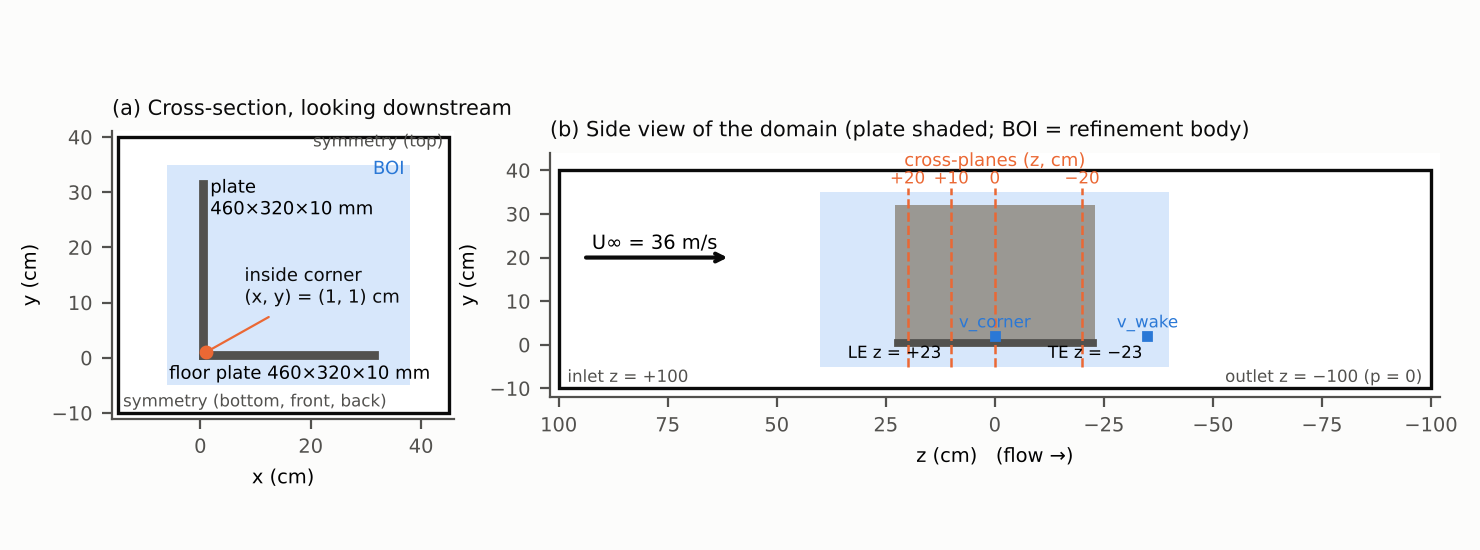
\includegraphics[width=\textwidth]{fig2_1.png}
\caption{Geometry, domain, BOI, cross-planes and monitor points.}
\label{fig:geom}
\end{figure}

\begin{table}[htbp]
\centering
\small
\begin{tabularx}{\textwidth}{@{}p{0.17\textwidth}p{0.33\textwidth}X@{}}
\toprule
Item & Mid-semester & Final \\
\midrule
Model & T-shape in small box & L-shaped junction \\
Side faces & No-slip walls & Symmetry \\
Inlet / outlet & 36\,m/s / 0\,Pa & 36\,m/s, $I = 1\%$, $\mu_t/\mu = 10$ / 0\,Pa \\
Outlet backflow & Turbulence $10^{-14}$ & $I = 5\%$, $\mu_t/\mu = 10$ \\
Mesh & 10\,mm tetrahedral, no inflation & 0.53--2.53\,M cells, 25 prism layers \\
Solver & SIMPLE, relaxation 0.1/0.2 & Coupled, pseudo-transient, second order \\
Verification & None & Monitor histories, mass balance, grid study \\
\bottomrule
\end{tabularx}
\caption[Settings before and after the mid-semester evaluation.]{Settings before and after the mid-semester evaluation. Air: $\rho = 1.225$\,kg/m$^3$, $\mu = 1.7894\times10^{-5}$\,kg/(m\,s); SST $k$--$\omega$; no-slip L surfaces (ANSYS Inc., 2024).}
\label{tab:settings}
\end{table}

The mesh (Figure~\ref{fig:mesh}) uses tetrahedra and wall-adjacent prisms, with a 50\,mm global size. Fine-grid face and BOI sizes are 5 and 12\,mm. Inflation is specified on all eight L faces: 0.01\,mm first layer, 25 layers and growth 1.2, giving a nominal total thickness of about 4.7\,mm. At the junction this is the prescribed inflation, not evidence that every layer retains its nominal thickness through the corner. Only face and BOI sizes were changed between grids; inflation and global size remained fixed.

\textbf{Mesh quality.} The fine mesh contains 2,528,284 cells. Maximum/mean skewness are 0.800/0.216; minimum/mean orthogonal quality are about 0.0064/0.764. About 2,660 cells (0.1\%) have orthogonal quality below 0.0156, at the outer free edge of the floor near $x \approx 0.318$\,m, away from the inside junction. The maximum aspect ratio is about 2,855 in the prism layers. These local defects remain a limitation despite acceptable global monitors and $y^+$.

\begin{figure}[htbp]
\centering
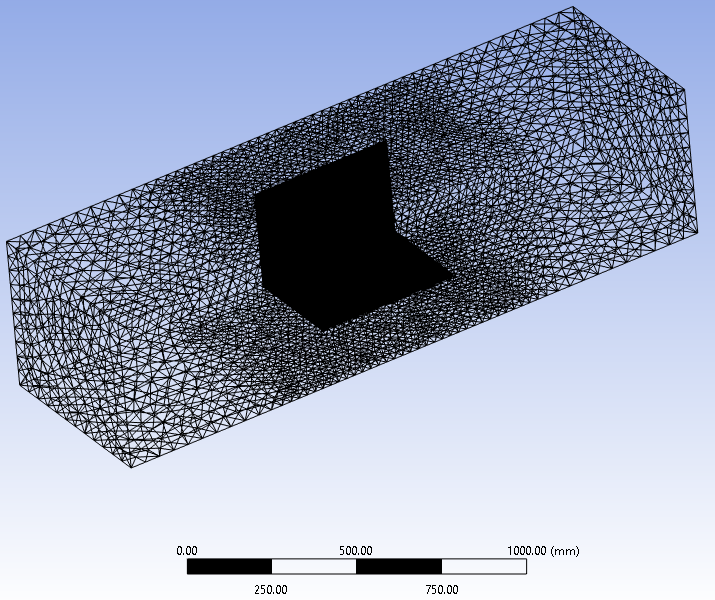
\includegraphics[width=0.78\textwidth]{fig2_2.png}
\caption[Fine mesh of the model and enclosure.]{Fine mesh of the L-shaped model inside the enclosure (ANSYS Meshing 2024 R1; 2,528,284 elements, 848,165 nodes). Surface mesh on the enclosure faces; cells cluster around the L inside the BOI.}
\label{fig:mesh}
\end{figure}

\textbf{Domain size.} The domain cross-section (0.30\,m$^2$) is blocked by about 2.1\% by the two blunt 10\,mm edges. The top symmetry plane lies about 80\,mm above the free edge of the vertical plate, and the outlet is 0.77\,m (1.7$L$) behind the TE. These distances are adequate for the corner flow over the plate, but they limit the accuracy of the far-wake values (Section~\ref{sec:verif}).

\section{Analysis}
Let $s = 0.23 - z$ be distance downstream from the LE, $d$ the distance normal to a wall, and $U = |\mathbf{u}|$ the exported velocity magnitude; $u$, $v$ and $w$ remain Cartesian components. Drag on all eight L faces (pressure and viscous contributions) is projected along $(0, 0, -1)$: $\Cd = F_D/(\tfrac12\rho\Uinf^2 A_\mathrm{ref})$, with $A_\mathrm{ref} = 0.46\times0.32 = 0.1472$\,m$^2$, the side area of one plate. The corner and wake monitors are velocity magnitudes at $(0.02, 0.02, 0)$ and $(0.02, 0.02, -0.35)$\,m.

At $z = 0$, profiles normal to each wall lie 240\,mm (far) or 10\,mm (near) from the other wall; a fifth profile follows the bisector. For far profiles, $U_e$ is the mean for $d > 35$\,mm and $\dn$ is interpolated at $0.99U_e$. The script integrates the sampled profile to $d = 50$\,mm with $q = \min[1, \max(0, U/U_e)]$: $\delta^* = \int(1-q)\,\mathrm{d}d$ and $\theta = \int q(1-q)\,\mathrm{d}d$. Thus these are finite-range, speed-based estimates; near profiles without a plateau are not assigned conventional thicknesses. Bisector distance is $(x + y - 0.02)/\sqrt{2}$.

Cross-planes at $z = +0.20$, $+0.10$, 0 and $-0.20$\,m correspond to $s = 30$, 130, 230 and 430\,mm. Exported nodal fields are linearly interpolated onto a $241\times241$ grid over 0--60\,mm from each inner wall. Positive and negative $\omega_z$ are integrated separately over finite samples, excluding the first 2\,mm next to either wall. Wall comparisons use corner (0--4\,mm), downwash (15--30\,mm) and reference (60--150\,mm) bands. $\Cf$ uses wall-shear magnitude divided by $\tfrac12\rho\Uinf^2$; the signed streamwise shear identifies reversal.

% ------------------------------------------------------------
\chapter{Results and Discussion}
\section{Verification}\label{sec:verif}
Over the final 200 iterations, drag half-range is $\le 0.05\%$ of its mean and velocity-monitor half-ranges are $\le 0.9\%$ (Figure~\ref{fig:monitors}). The fine-grid corner and wake values retain bounded oscillations, not a strictly steady fixed point. Fine-grid residuals plateau at approximately $3\times10^{-3}$ (continuity), $10^{-6}$ (velocity), $1.5\times10^{-3}$ ($k$) and $3\times10^{-4}$ ($\omega$, specific dissipation rate); not all meet the $10^{-6}$ stopping criterion. Mass imbalance is below $2\times10^{-4}\%$ on all grids, and maximum $y^+$ is 0.77--0.93.

\begin{figure}[htbp]
\centering
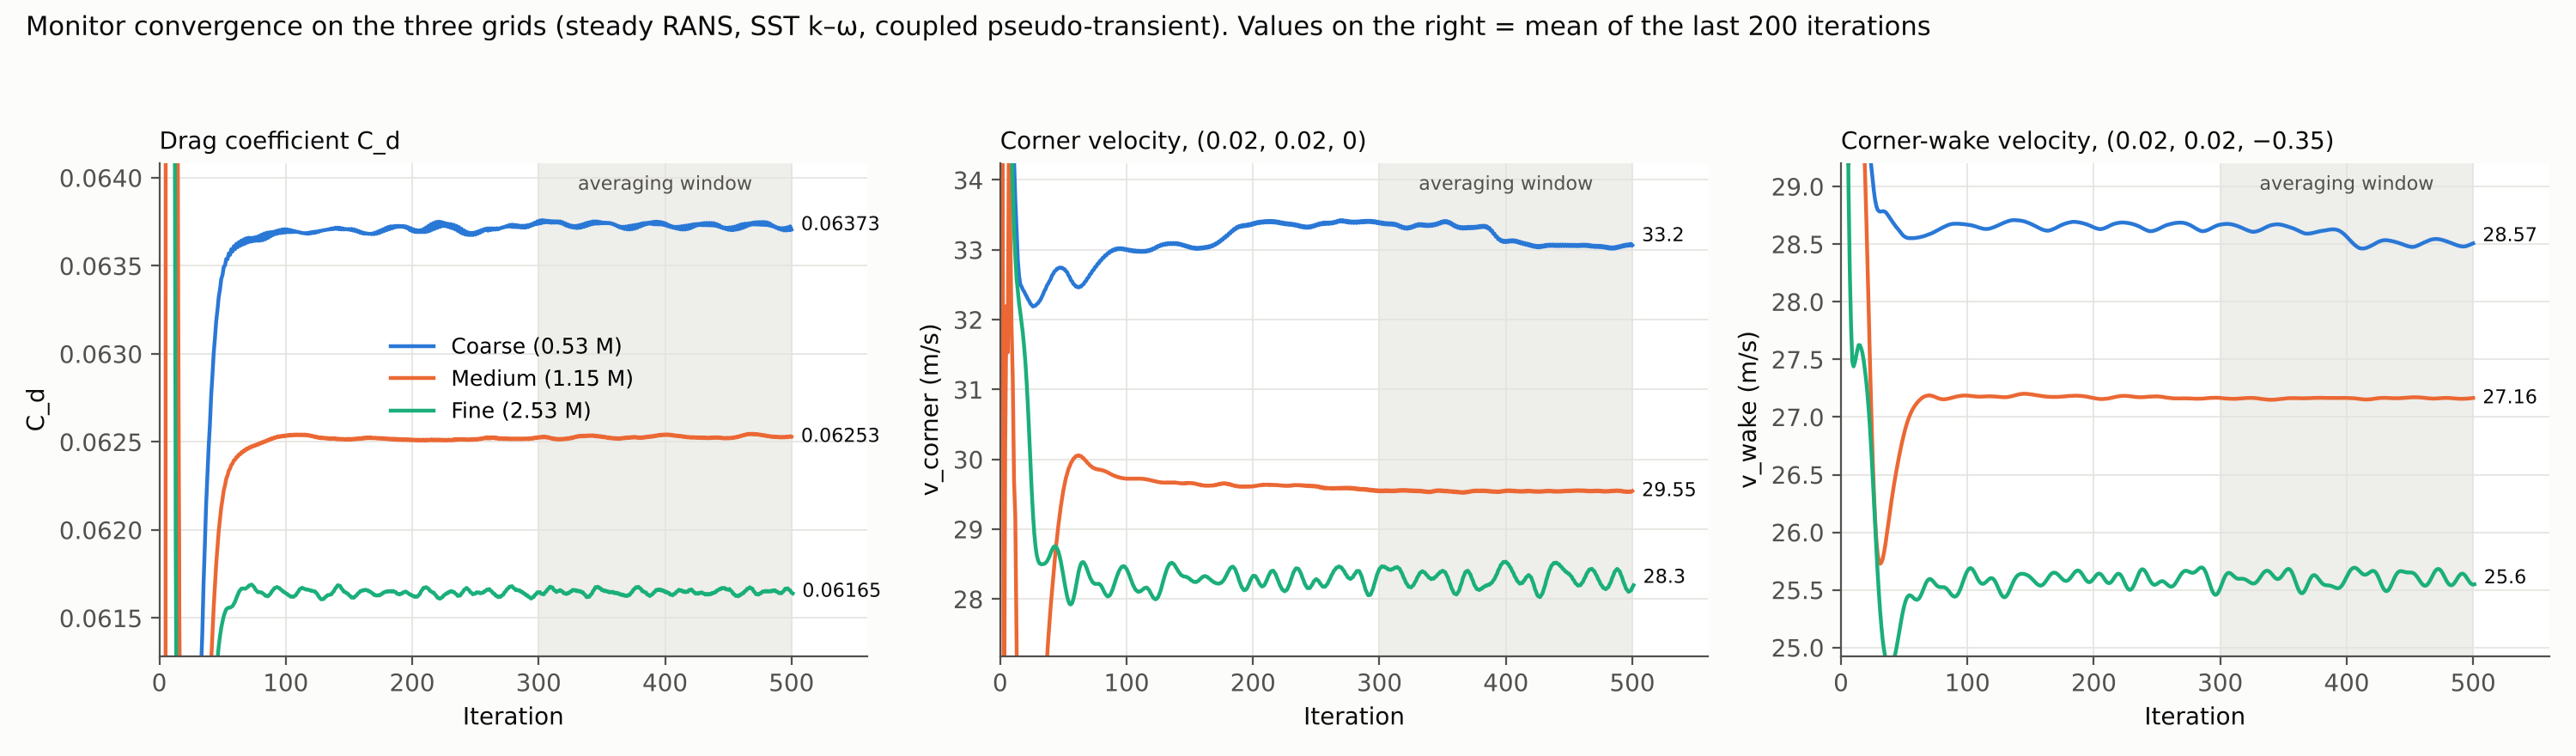
\includegraphics[width=\textwidth]{fig3_1.png}
\caption[Monitor histories on the three grids.]{Monitor histories; shaded bands mark the final 200 iterations. The reference values were corrected during the fine-grid run; fine-grid $\Cd$ before iteration 178 is rescaled to the corrected reference values.}
\label{fig:monitors}
\end{figure}

\begin{table}[htbp]
\centering
\small
\begin{tabularx}{\textwidth}{@{}p{0.25\textwidth}llllX@{}}
\toprule
Grid; face / BOI (mm) & $N$ (M) & $h$ (mm) & $\Cd$ & $U_\mathrm{corner}$ & $U_\mathrm{wake}$ \\
\midrule
Coarse; 10.6 / 25.5 & 0.529 & 10.41 & 0.063731 & 33.195 & 28.569 \\
Medium; 7.3 / 17.5  & 1.150 & 8.04  & 0.062529 & 29.546 & 27.162 \\
Fine; 5.0 / 12.0    & 2.528 & 6.18  & 0.061649 & 28.304 & 25.600 \\
\midrule
Medium-to-fine change & -- & -- & 1.43\% & 4.4\% & 6.1\% \\
Apparent order $p$    & -- & -- & 1.25 & 4.2 & Not reliable \\
Extrapolated value    & -- & -- & 0.0594 & 27.69 & -- \\
Fine-grid GCI         & -- & -- & 4.6\% & 2.7\% ($\approx$8\% with $p=2$) & Not defined \\
\bottomrule
\end{tabularx}
\caption[Three-grid study: final-200-iteration means and GCI.]{Three-grid study: final-200-iteration means; velocities in m/s. Effective ratios $r_{21}\approx1.300$ and $r_{32}\approx1.295$.}
\label{tab:grid}
\end{table}

Drag changes by 1.43\% from medium to fine, and the extrapolated value is 3.7\% below the fine-grid value (Figure~\ref{fig:grid}). GCI estimates are conditional because refinement is not uniform. For the corner monitor the medium-to-fine change is 4.4\%; because the apparent order $p = 4.2$ exceeds the formal order of the scheme, the 2.7\% GCI should be read as a lower bound, and limiting $p$ to 2 (Roache, 1998) gives about 8\%. Wake values decrease monotonically, but successive differences grow (1.407 to 1.562\,m/s; ratio $\approx 1.11$), so no reliable asymptotic GCI is obtained. Its 6.1\% medium-to-fine difference is not a quantified uncertainty; the short outlet distance (Section~2.1) may contribute. Subsequent results use the fine grid.

\begin{figure}[htbp]
\centering
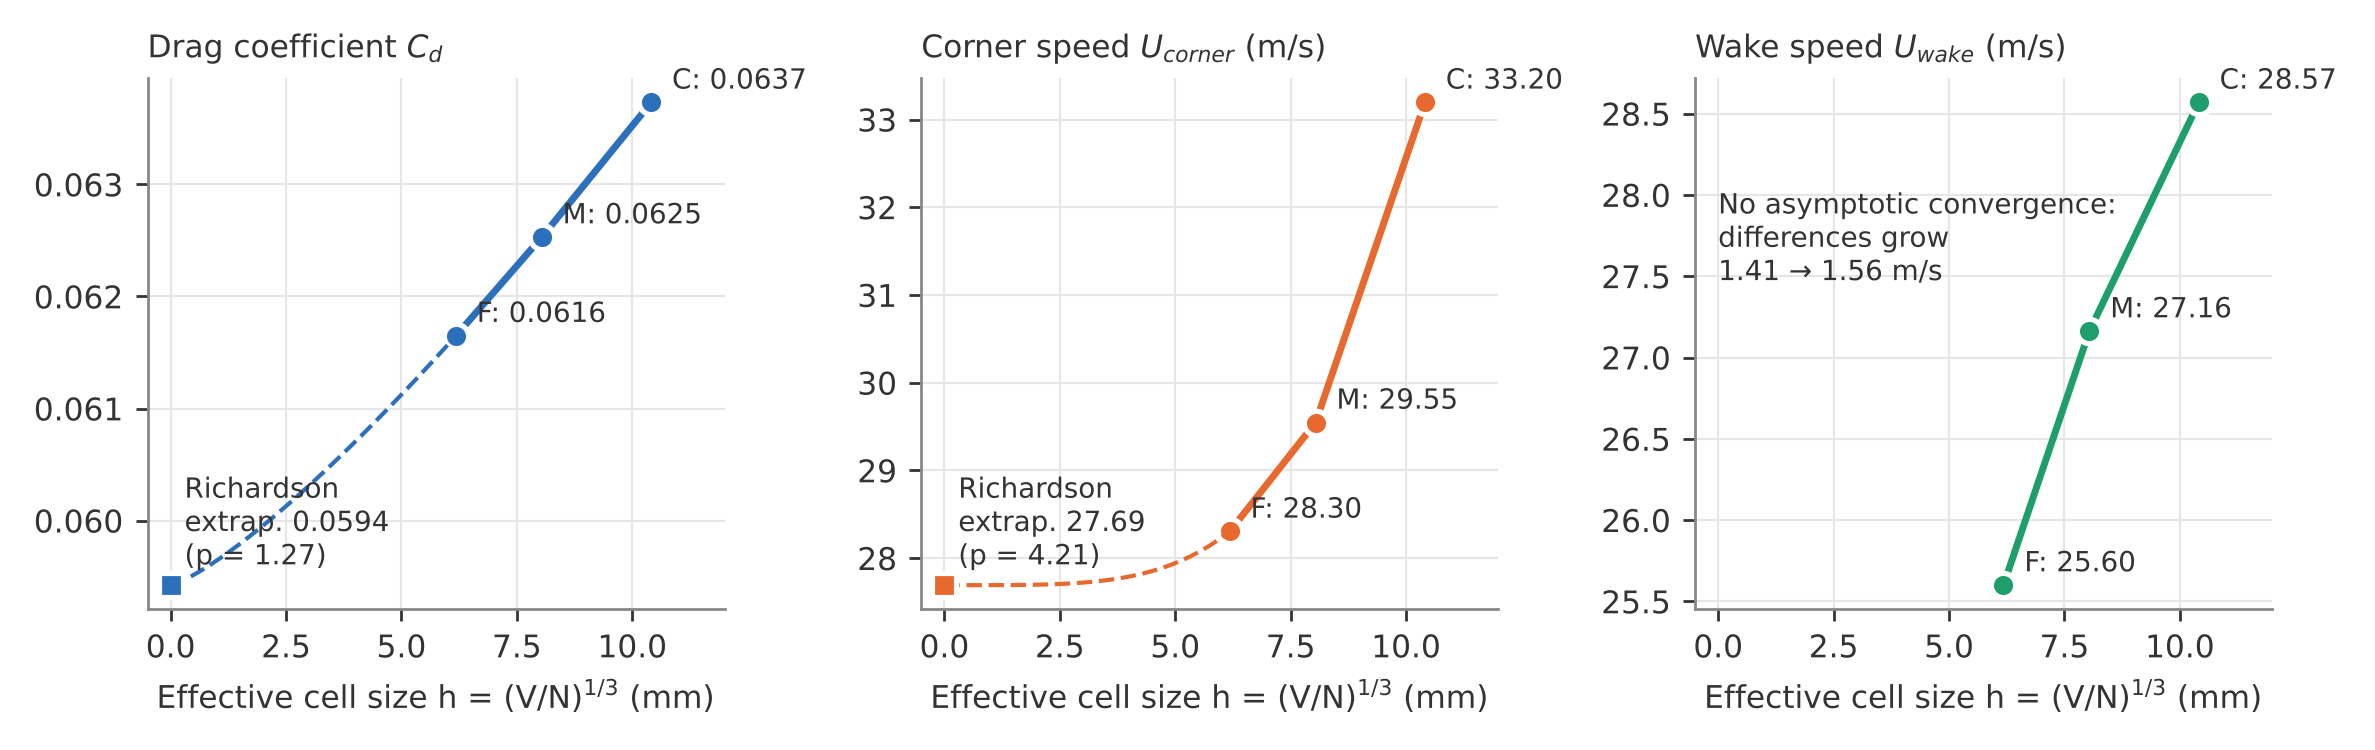
\includegraphics[width=\textwidth]{fig3_2.png}
\caption[Grid convergence of the monitored quantities.]{Final-200-iteration means versus effective cell size for the coarse (C), medium (M) and fine (F) grids. Dashed curves and squares show the Richardson extrapolation $h\to0$ (Celik et al., 2008). $\Cd$ and $U_\mathrm{corner}$ converge monotonically; $U_\mathrm{wake}$ shows growing differences and has no asymptotic estimate.}
\label{fig:grid}
\end{figure}

\section{Leading edge of the junction}\label{sec:le}
The inlet total pressure is 819\,Pa (794\,Pa dynamic plus 25\,Pa static). The node-averaged maximum pressure on the L is 837\,Pa, 2\% above the inlet total pressure. Since the static pressure cannot physically exceed the upstream total pressure, this overshoot is a local discretisation error at the sharp stagnation edge and indicates the numerical error there. Iso-surfaces place the largest stagnation region at the inside corner of the blunt front face, where both plates obstruct the oncoming fluid. The node-averaged peak speed is $1.24\Uinf$; larger isolated cell peaks are not representative of the bulk flow. Acceleration around the square edges is followed by separation. Reversed floor shear persists 70--77\,mm downstream from the LE far from the plate but only 40--50\,mm within 30\,mm of it (Figure~\ref{fig:cf}a).

\section{Boundary layers far from and near the junction}
Far from the junction the boundary layers are alike at mid-length: $\dn = 25.6$ and 26.0\,mm, $\delta^* = 6.12$ and 6.34\,mm, $\theta = 3.69$ and 3.86\,mm, and $H = 1.66$ and 1.64 for floor and plate respectively. These thicknesses exceed the flat-plate estimate $0.37 s\,Re_s^{-1/5} \approx 6$\,mm at $s = 0.23$\,m (Schlichting and Gersten, 2017). $H$ exceeds the equilibrium value 1.3--1.4, consistent with recovery after leading-edge separation. $U_e \approx 37.4$\,m/s is about 4\% above the inlet speed. This speed-up is consistent with the combined blockage of the blunt edges (2.1\% of the domain cross-section) and of the displacement thickness on the four wetted faces (about $1.28\,\mathrm{m}\times6.2\,\mathrm{mm}\approx2.6\%$).

\begin{figure}[htbp]
\centering
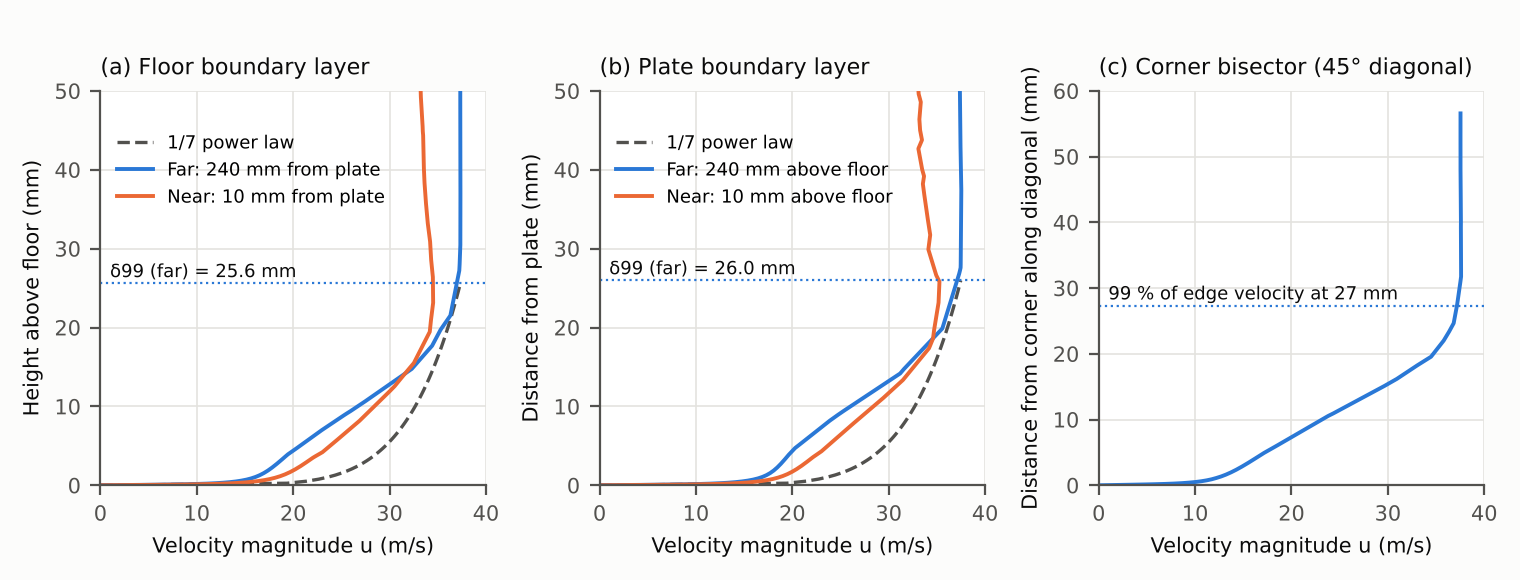
\includegraphics[width=\textwidth]{fig3_3.png}
\caption[Mid-length boundary-layer and corner-bisector profiles.]{Velocity-magnitude profiles at mid-length, far from (240\,mm) and near (10\,mm) the other wall, and along the corner bisector. The plotted $u$ denotes speed $U$, not the Cartesian $x$-component.}
\label{fig:profiles}
\end{figure}

Near-corner profiles are fuller close to the wall: about 28.4\,m/s at $d = 10$\,mm compared with 26.0--26.7\,m/s far away. They do not reach an independent outer plateau because they remain in the other wall's boundary layer. Along the bisector, 99\% of $U_e$ is reached at 27.3\,mm, versus the geometric scale $\sqrt{2}\,\dn \approx 36$\,mm. This point is only $27.3/\sqrt{2}\approx19$\,mm from each wall, less than $\dn$, so the corner region carries more momentum than either boundary layer alone would suggest. This comparison is consistent with momentum redistribution by the secondary flow (Section~\ref{sec:sec}), but is not a rigorous superposition model.

\section{Vorticity at the corner}
The floor boundary layer carries $\omega_x < 0$ and the plate boundary layer $\omega_y > 0$, with wall magnitudes of order $10^{5}$\,s$^{-1}$. At $z = 0$, the $\omega_x$ layer thins towards the plate and the $\omega_y$ layer weakens towards the floor (Figure~\ref{fig:wxy}). This shows interaction between the two wall-vorticity distributions, but contours alone do not trace connected vortex lines.

\begin{figure}[htbp]
\centering
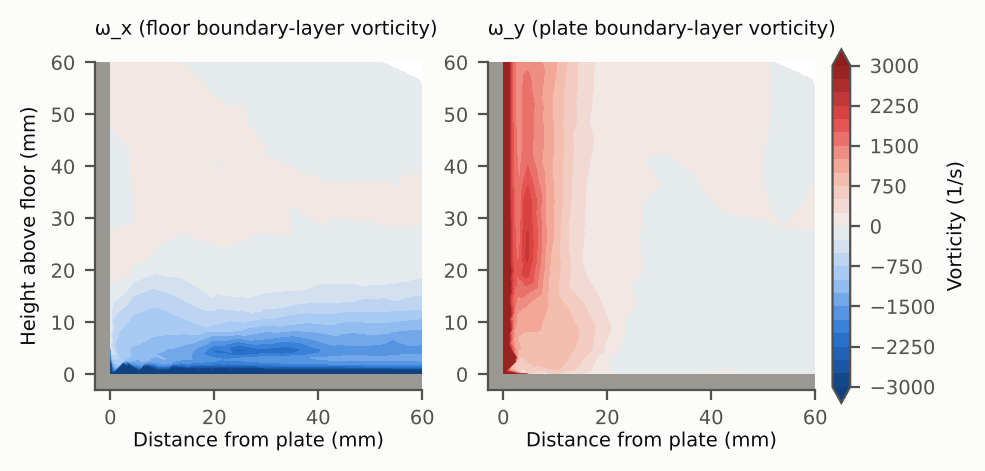
\includegraphics[width=0.88\textwidth]{fig3_4.png}
\caption[Floor and plate vorticity components at $z = 0$.]{Floor-associated $\omega_x$ and plate-associated $\omega_y$ at $z = 0$. The $\pm3{,}000$\,s$^{-1}$ plotting range resolves the outer layers and does not represent the much larger wall extrema.}
\label{fig:wxy}
\end{figure}

For incompressible mean flow, the streamwise vorticity equation may be written schematically as
\begin{equation}
(\mathbf{u}\cdot\nabla)\,\omega_z = \omega_x\frac{\partial w}{\partial x} + \omega_y\frac{\partial w}{\partial y} + \omega_z\frac{\partial w}{\partial z} + \nu\nabla^2\omega_z - \big[\nabla\times(\nabla\cdot\mathbf{R})\big]_z ,
\label{eq:vort}
\end{equation}
where $R_{ij} = \langle u_i' u_j' \rangle$ is the time-averaged Reynolds-stress tensor. The first two right-hand terms represent tilting, the third stretching, and the remaining terms viscous and turbulent-stress contributions. Independently, $\nabla\cdot\boldsymbol{\omega} = 0$ implies $\partial\omega_z/\partial z = -(\partial\omega_x/\partial x + \partial\omega_y/\partial y)$.

The solenoidal condition constrains the spatial field but does not establish which transport term in Eq.~\eqref{eq:vort} creates the corner vorticity. A term-by-term budget or vortex-line/pathline analysis was not performed. The interpretation of leading-edge tilting is therefore based on the joint evidence of vorticity, separation and cross-flow, rather than a measured transport balance.

\begin{figure}[htbp]
\centering
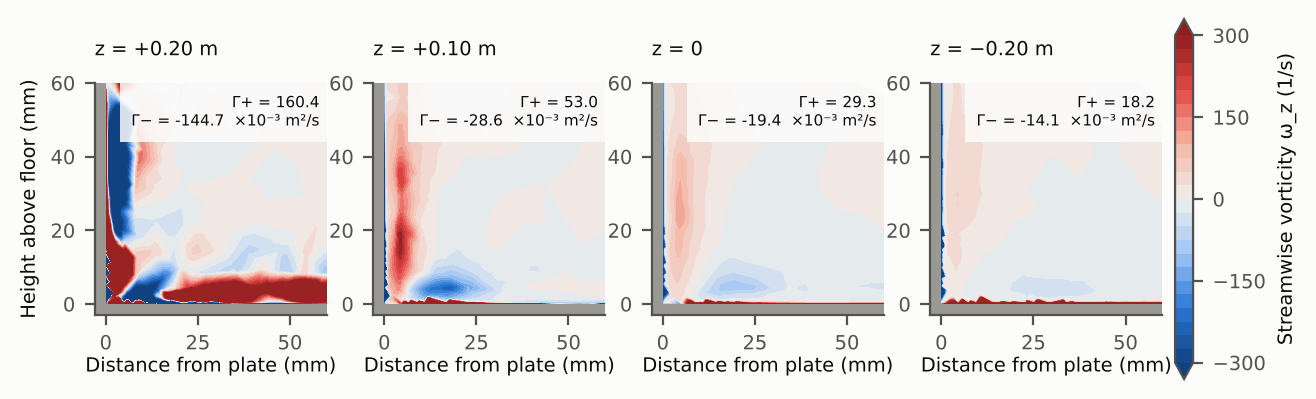
\includegraphics[width=\textwidth]{fig3_5.png}
\caption[Streamwise vorticity on four cross-planes.]{Streamwise vorticity at $z = +0.20$, $+0.10$, 0 and $-0.20$\,m ($s = 30$, 130, 230 and 430\,mm). Colour limits are $\pm300$\,s$^{-1}$; leading-edge extremes exceed this range.}
\label{fig:wz}
\end{figure}

Inside the leading-edge separation bubble ($z = +0.20$\,m), $\omega_z$ is strong and patchy (Figure~\ref{fig:wz}). Farther downstream, positive vorticity remains predominantly beside the plate and negative vorticity above the floor, centred roughly 5--20\,mm from the walls. The topology is consistent with a counter-rotating pair, but the two signed circulations are unequal, particularly at $z = +0.10$\,m; the flow should not be described as quantitatively symmetric.

\begin{table}[htbp]
\centering
\small
\begin{tabular}{@{}llllll@{}}
\toprule
$z$ (m) & $s$ (mm) & $\Gamma^+$ & $\Gamma^-$ & $\Gamma^+ + |\Gamma^-|$ & $\Gamma^+/|\Gamma^-|$ \\
\midrule
$+0.20$ & 30  & 160.4 & $-144.7$ & 305.1 & 1.11 \\
$+0.10$ & 130 & 53.0  & $-28.6$  & 81.6  & 1.85 \\
0       & 230 & 29.3  & $-19.4$  & 48.7  & 1.51 \\
$-0.20$ & 430 & 18.2  & $-14.1$  & 32.3  & 1.29 \\
\bottomrule
\end{tabular}
\caption[Circulation in the sampled corner window.]{Signed and total unsigned circulation, in $10^{-3}$\,m$^2$/s, from the same $60\times60$\,mm window with the 2\,mm wall strips excluded.}
\label{tab:circ}
\end{table}

Across the sampled planes, positive circulation falls by $160.4/18.2 \approx 8.8$ times and negative-circulation magnitude by $144.7/14.1 \approx 10.3$ times. Their sum falls by $305.1/32.3 \approx 9.5$ times. These are changes between $s = 30$ and 430\,mm, not measurements exactly at the LE and TE.

\begin{figure}[htbp]
\centering
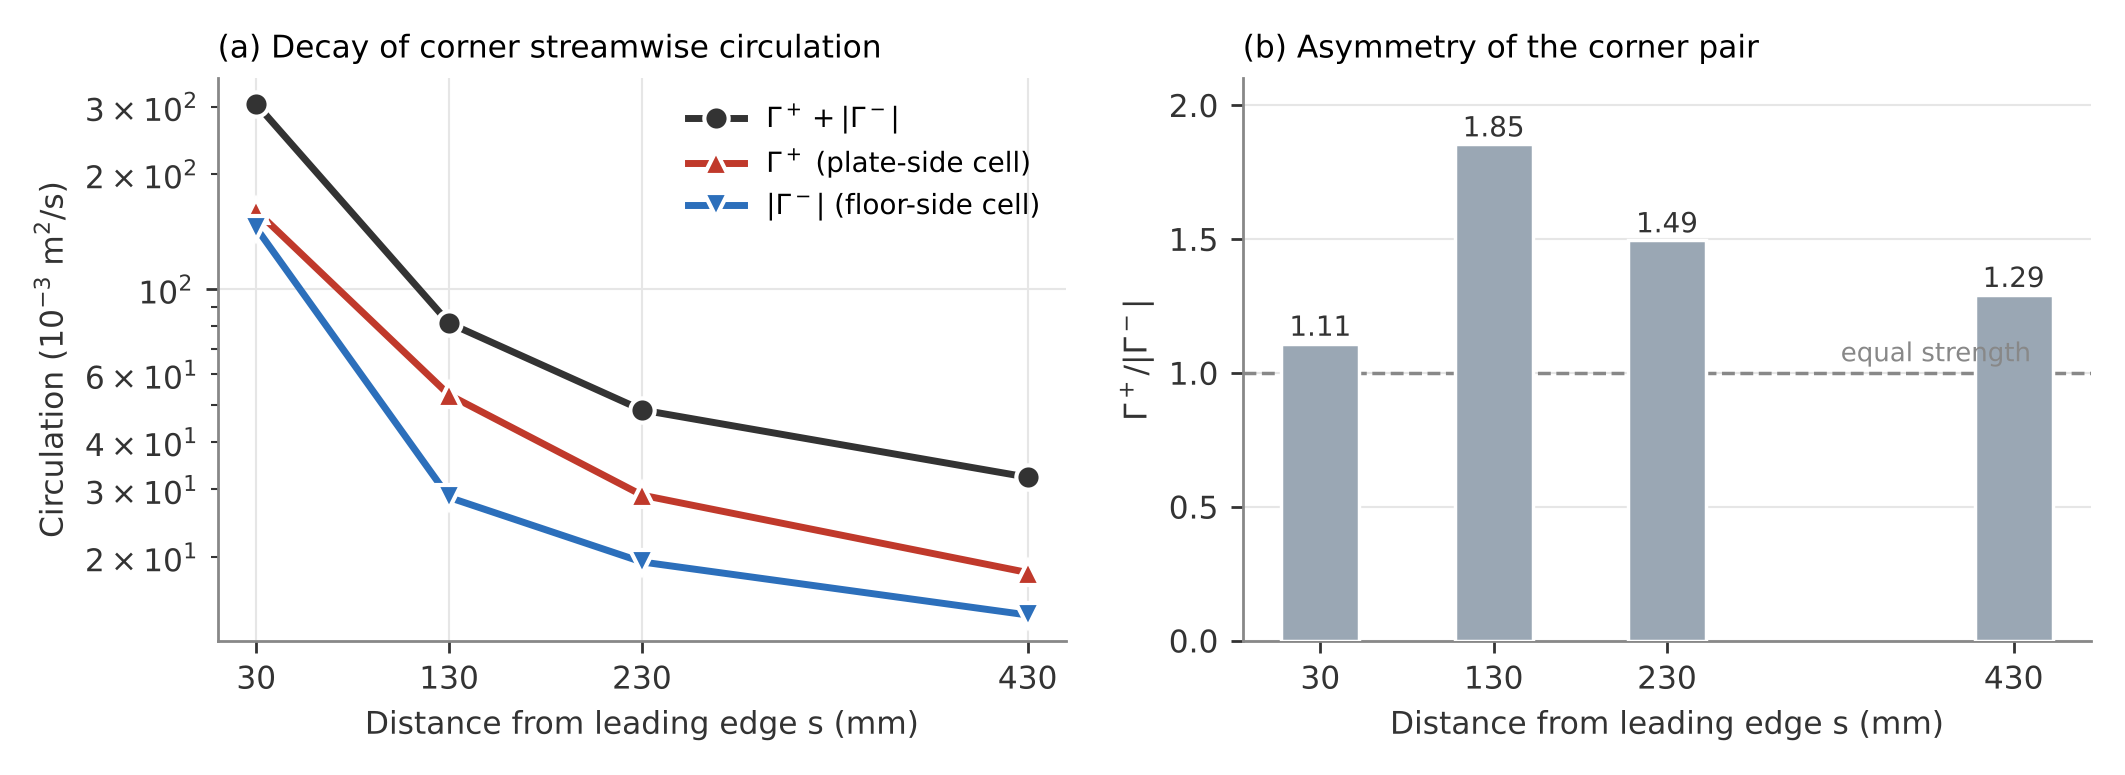
\includegraphics[width=\textwidth]{fig3_6.png}
\caption[Decay and asymmetry of the corner circulation.]{(a) Signed and total circulation in the $60\times60$\,mm corner window versus distance from the leading edge (logarithmic scale). (b) Ratio $\Gamma^+/|\Gamma^-|$; the dashed line marks equal strength.}
\label{fig:circ}
\end{figure}

Figure~\ref{fig:circ} shows that most of the reduction occurs between $s = 30$ and 130\,mm (a factor of 3.7 in total circulation), where the leading-edge separation bubble reattaches (Section~\ref{sec:le}); between $s = 130$ and 430\,mm the total falls by a further factor of only 2.5. The plate-side cell ($\Gamma^+$) is stronger at every station ($\Gamma^+/|\Gamma^-| = 1.11$--1.85). This is consistent with the shorter floor separation bubble near the plate and with the asymmetric skin-friction enhancement in Section~\ref{sec:cf}.

The downstream reduction is consistent with weakening and redistribution of leading-edge-generated vorticity. Diffusion may contribute, but flux through the finite window, convection, stretching and tilting have not been separated. The result therefore supports a leading-edge-related, first-kind secondary-flow interpretation without proving that turbulent diffusion alone causes the decay.

\section{Secondary flow and mixing in the corner}\label{sec:sec}
Figure~\ref{fig:isovels} shows the cross-flow associated with the corner pair. At $z = +0.10$\,m and 0, vectors within approximately 3\,mm of each wall point towards the corner (0.1--0.46\,m/s), while vectors along the bisector point away from it (0.07--0.28\,m/s). Low-momentum fluid is swept along the walls into the corner and lifted along the bisector. On the outer side of each cell, faster fluid is brought towards the wall about 15--30\,mm from the corner. The floor-side circulation has the same sense as a horseshoe-vortex leg (Simpson, 2001). The bisector outflow is weak and confined close to the corner; over the corner region as a whole the high-momentum downwash on either side dominates, which is why the near-corner profiles in Figure~\ref{fig:profiles} are fuller than the far profiles.

\begin{figure}[htbp]
\centering
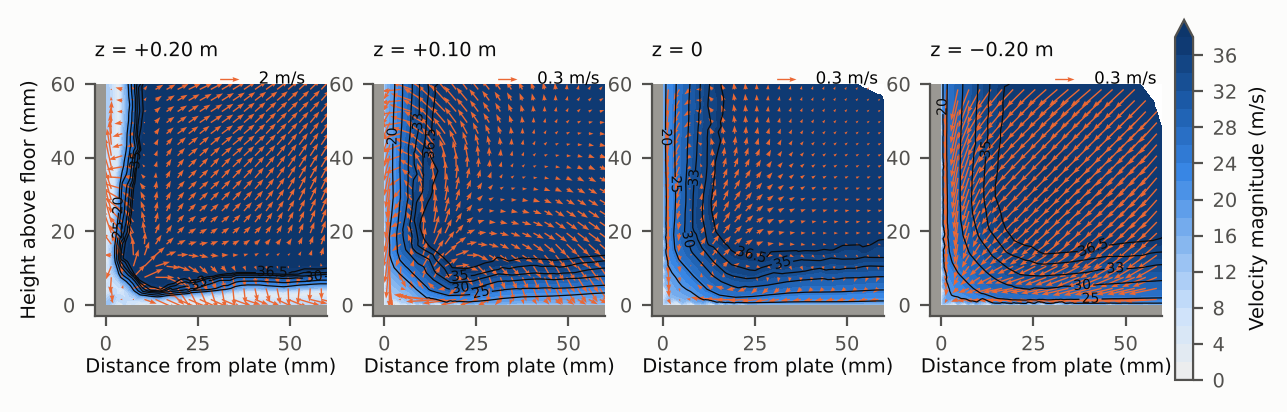
\includegraphics[width=\textwidth]{fig3_7.png}
\caption[Isovels and cross-flow vectors on four cross-planes.]{Isovels (black, m/s) and cross-flow vectors on the four planes. The first panel uses a 2\,m/s reference arrow; the others use 0.3\,m/s. Vector lengths must be compared with their own reference scale.}
\label{fig:isovels}
\end{figure}

The isovels bend towards the walls beside the corner, consistent with the fuller near-wall profiles in Figure~\ref{fig:profiles} and the shorter bisector distance to 99\% of the edge speed. High-momentum transport is towards the walls on the downwash sides of the cells; it is not directed into the corner along the bisector, where the intermediate-plane vectors point outward.

At $z = +0.20$\,m the maximum cross-flow in the sampled window is about 3.5\,m/s (nearly 10\% of $\Uinf$) and is dominated by outward displacement from the blunt leading edge. At $z = -0.20$\,m the cross-flow converges towards the walls ahead of the trailing edge. Thus the intermediate-plane circulation pattern should not be extrapolated unchanged to every streamwise station.

These velocity and vorticity fields demonstrate mean momentum redistribution. They do not quantify turbulent mixing rates or resolve unsteady vortex shedding; the calculation is steady RANS, and the remaining iterative oscillations are not a physical time history.

\section{Wall shear stress}\label{sec:cf}
The secondary flow leaves a clear imprint on skin friction (Figure~\ref{fig:cf}). Within 4\,mm of the corner, $\Cf$ is about 30--50\% lower than in the reference band 60--150\,mm away. For example, on the floor at $z = +0.10$\,m it is $1.05\times10^{-3}$, compared with $2.16\times10^{-3}$ in the reference band. Part of this reduction is geometric: the velocity gradient, and hence the wall shear, vanishes towards a $90^\circ$ corner because both walls retard the flow. The secondary flow modifies the distribution around this, sweeping low-momentum fluid along the walls into the corner and producing the downwash band of increased $\Cf$.

\begin{figure}[htbp]
\centering
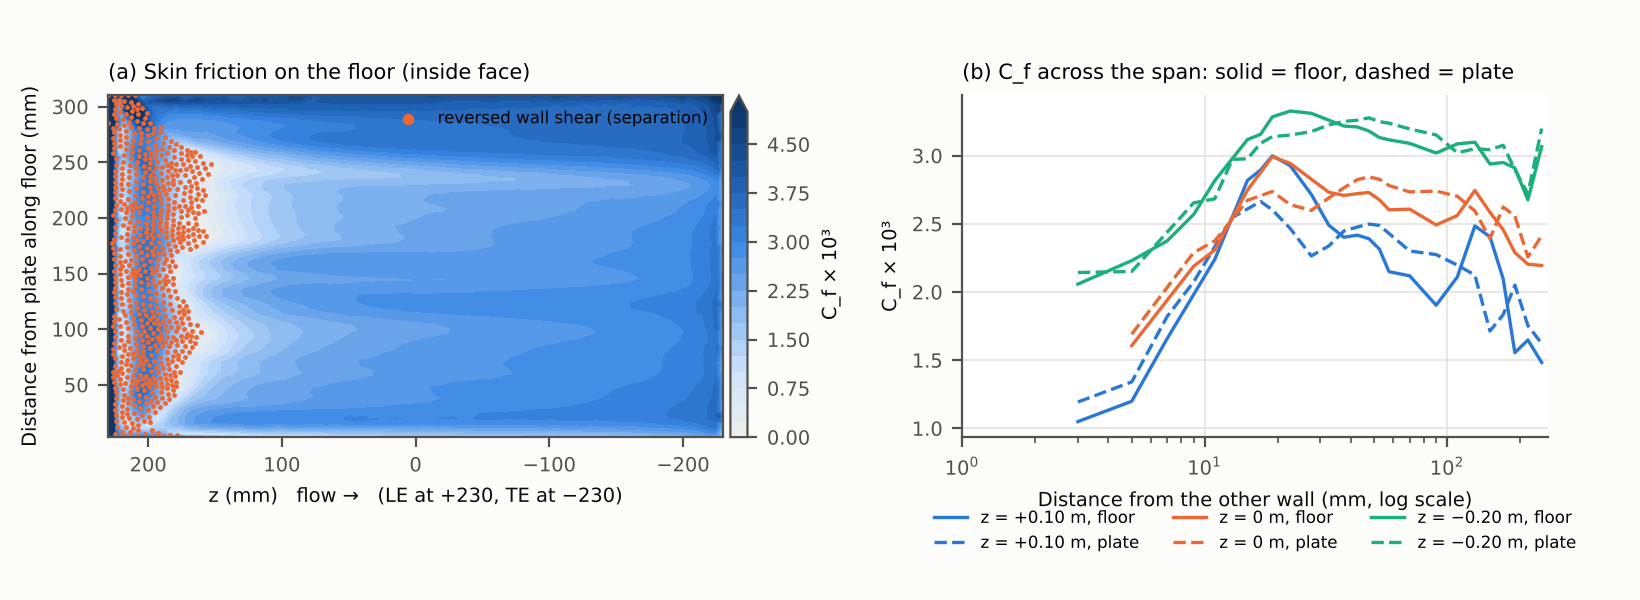
\includegraphics[width=\textwidth]{fig3_8.png}
\caption[Skin-friction distribution and comparison across the span.]{(a) Skin-friction magnitude on the inside floor, with signed-shear reversal marked; (b) $\Cf$ versus distance from the other wall at three stations. Solid lines represent the floor and dashed lines the plate.}
\label{fig:cf}
\end{figure}

In the 15--30\,mm downwash band, the floor $\Cf$ is $2.86\times10^{-3}$ at $z = +0.10$\,m, 32\% above the reference-band mean; the plate increase there is about 13\%. The floor enhancement declines to approximately 12\% at $z = 0$ and 8\% at $z = -0.20$\,m, while the corresponding plate changes are about 0\% and 2\%. These differences are consistent with the unequal vortex strengths (Figure~\ref{fig:circ}b). Away from the corner, $\Cf$ increases downstream as the boundary layer recovers after separation.

\textbf{Relation to the reference experiment.} In Nakayama and Rahai (1984), a developed wall boundary layer arrives from upstream. Here both wall boundary layers start at the same blunt LE. The comparison is therefore qualitative: both flows show streamwise corner vorticity, momentum redistribution and local wall-shear changes. Agreement of these trends does not establish quantitative validation against that experiment.

% ------------------------------------------------------------
\chapter{Conclusions and Future Work}
\begin{enumerate}[label=\arabic*.,leftmargin=*,itemsep=6pt]
\item The corrected L-junction RANS model satisfies $y^+ < 1$ and global mass balance, with bounded final-iteration monitor variation. The fine-grid drag coefficient is $\Cd = 0.06165$; its estimated discretisation GCI is 4.6\% and the extrapolated value is 3.7\% lower. The corner-speed GCI is 2.7\%, but this relies on an apparent order (4.2) above the formal order; limiting the order to 2 gives about 8\%, comparable to the 4.4\% medium-to-fine change. These are discretisation estimates, not total uncertainties or experimental validation.
\item The wake-monitor velocity decreases monotonically from coarse to fine, but grid differences do not contract. The 6.1\% medium-to-fine difference is a sensitivity measure, not a reliable uncertainty estimate; further local refinement and a longer downstream domain are needed for a converged wake value.
\item The blunt LE produces the strongest stagnation region at the inside corner and a shorter separation bubble near the junction (40--50\,mm) than far from it (70--77\,mm). The mid-length layers remain much thicker than an equilibrium flat-plate estimate.
\item Vorticity contours and cross-flow vectors indicate a counter-rotating corner pair with unequal strengths; the plate-side cell is 1.1--1.9 times stronger at every station. The total unsigned circulation in the sampled window decreases about 9.5 times between $s = 30$ and 430\,mm, by a factor of 3.7 already within the first 130\,mm. Leading-edge tilting is a plausible interpretation; neither a complete vorticity budget nor vortex-line connectivity was demonstrated.
\item At intermediate stations, low-momentum fluid moves towards the corner along the walls and away along the bisector, while faster fluid moves towards the walls 15--30\,mm away, so that the corner region as a whole is fuller than either boundary layer alone. Corner skin friction is 30--50\% lower than the reference band, partly for geometric reasons; the adjacent floor enhancement reaches 32\% and diminishes downstream.
\end{enumerate}

{\small
\textbf{Limitations and future work.} SST cannot represent the Reynolds-stress-anisotropy mechanism of second-kind corner flow, which matters most downstream, where cross-flow falls from about 10\% to 1\% of $\Uinf$. The outlet is only 1.7$L$ behind the TE, the top boundary is about 80\,mm above the plate edge, and 0.1\% of cells have low orthogonal quality at the outer floor edge. Future work: an SST corner-flow correction or Reynolds-stress model, a longer domain with a refined corner wake, vortex lines and wake-recovery profiles, a pressure/viscous drag split, an incoming wall boundary layer for experimental comparison, and the NACA 0010 wing--body junction.
\par}

% ============================================================
%  REFERENCES (author--year, as cited in the text)
% ============================================================
\chapter*{References}
\addcontentsline{toc}{chapter}{References}
\thispagestyle{plain}
\markboth{References}{}
\begin{list}{}{\setlength{\leftmargin}{1.5em}\setlength{\itemindent}{-1.5em}\setlength{\itemsep}{6pt}}
\item ANSYS Inc. (2024). \emph{Ansys Fluent Theory Guide, Release 2024 R1.} ANSYS Inc., Canonsburg, PA.
\item Bradshaw, P. (1987). Turbulent secondary flows. \emph{Annual Review of Fluid Mechanics}, 19:53--74.
\item Celik, I. B., Ghia, U., Roache, P. J., Freitas, C. J., Coleman, H., and Raad, P. E. (2008). Procedure for estimation and reporting of uncertainty due to discretization in CFD applications. \emph{Journal of Fluids Engineering}, 130(7):078001.
\item Gessner, F. B. (1973). The origin of secondary flow in turbulent flow along a corner. \emph{Journal of Fluid Mechanics}, 58(1):1--25.
\item Menter, F. R. (1994). Two-equation eddy-viscosity turbulence models for engineering applications. \emph{AIAA Journal}, 32(8):1598--1605.
\item Nakayama, A. and Rahai, H. R. (1984). Measurements of turbulent flow behind a flat plate mounted normal to the wall. \emph{AIAA Journal}, 22(12):1817--1819.
\item Pope, S. B. (2000). \emph{Turbulent Flows.} Cambridge University Press, Cambridge.
\item Roache, P. J. (1998). \emph{Verification and Validation in Computational Science and Engineering.} Hermosa Publishers, Albuquerque, NM.
\item Saffman, P. G. (1992). \emph{Vortex Dynamics.} Cambridge University Press, Cambridge.
\item Schlichting, H. and Gersten, K. (2017). \emph{Boundary-Layer Theory.} Springer, Berlin, 9th edition.
\item Simpson, R. L. (2001). Junction flows. \emph{Annual Review of Fluid Mechanics}, 33:415--443.
\end{list}

\end{document}
